\documentclass[12pt,twoside]{article}
\usepackage[dvipsnames]{xcolor}
\usepackage{tikz,graphicx,amsmath,amsfonts,amscd,amssymb,bm,cite,epsfig,epsf,url}
\usepackage[hang,flushmargin]{footmisc}
\usepackage[colorlinks=true,urlcolor=blue,citecolor=blue]{hyperref}
\usepackage{amsthm,multirow,wasysym,appendix}
\usepackage{array,subcaption} 
% \usepackage[small,bf]{caption}
\usepackage{bbm}
\usepackage{pgfplots}
\usetikzlibrary{spy}
\usepgfplotslibrary{external}
\usepgfplotslibrary{fillbetween}
\usetikzlibrary{arrows,automata}
\usepackage{thmtools}
\usepackage{blkarray} 
\usepackage{textcomp}
\usepackage[left=0.8in,right=1.0in,top=1.0in,bottom=1.0in]{geometry}

\usepackage{times}
\usepackage{amsfonts}
\usepackage{amsmath}
\usepackage{latexsym}
\usepackage{color}
\usepackage{graphics}
\usepackage{enumerate}
\usepackage{amstext}
\usepackage{blkarray}
\usepackage{url}
\usepackage{epsfig}
\usepackage{bm}
\usepackage{hyperref}
\hypersetup{
    colorlinks=true,
    linkcolor=blue,
    filecolor=magenta,      
    urlcolor=blue,
}
\usepackage{textcomp}
\usepackage[left=0.8in,right=1.0in,top=1.0in,bottom=1.0in]{geometry}
\usepackage{mathtools}
\usepackage{minted}


%% Probability operators and functions
%
% \def \P{\mathrm{P}}
\def \P{\mathrm{P}}
\def \E{\mathrm{E}}
\def \Var{\mathrm{Var}}
\let\var\Var
\def \Cov {\mathrm{Cov}} \let\cov\Cov
\def \MSE {\mathrm{MSE}} \let\mse\MSE
\def \sgn {\mathrm{sgn}}
\def \R {\mathbb{R}}
\def \C {\mathbb{C}}
\def \N {\mathbb{N}}
\def \Z {\mathbb{Z}}
\def \cV {\mathcal{V}}
\def \cS {\mathcal{S}}
\DeclareMathOperator*{\argmin}{arg\,min}
\DeclareMathOperator*{\argmax}{arg\,max}
\newcommand{\red}[1]{\textcolor{red}{#1}}
\newcommand{\blue}[1]{\textcolor{blue}{#1}}
\newcommand{\green}[1]{\textcolor{ForestGreen}{ #1}}
\newcommand{\fuchsia}[1]{\textcolor{RoyalPurple}{ #1}}

%
%% Probability distributions
%
%\def \Bern    {\mathrm{Bern}}
%\def \Binom   {\mathrm{Binom}}
%\def \Exp     {\mathrm{Exp}}
%\def \Geom    {\mathrm{Geom}}
%\def \Norm    {\mathcal{N}}
%\def \Poisson {\mathrm{Poisson}}
%\def \Unif    {\mathrm {U}}
%
\newcommand{\bdb}[1]{\textcolor{red}{#1}}

\newcommand{\ml}[1]{\mathcal{ #1 } }
\newcommand{\wh}[1]{\widehat{ #1 } }
\newcommand{\wt}[1]{\widetilde{ #1 } }
\newcommand{\conj}[1]{\overline{ #1 } }
\newcommand{\rnd}[1]{\tilde{ #1 } }
\newcommand{\rv}[1]{ \rnd{ #1}  }
\newcommand{\rx}{\rnd{ x}  }
\newcommand{\ry}{\rnd{ y}  }
\newcommand{\ra}{\rnd{ a}  }
\newcommand{\rb}{\rnd{ b}  }
\newcommand{\rpc}{\widetilde{ pc}  }

\def \cnd {\, | \,}
\def \Id { I }
\def \J {\mathbf{1}\mathbf{1}^T}

\newcommand{\op}[1]{\operatorname{#1}}
\newcommand{\setdef}[2]{ := \keys{ #1 \; | \; #2 } }
\newcommand{\set}[2]{ \keys{ #1 \; | \; #2 } }
\newcommand{\sign}[1]{\op{sign}\left( #1 \right) }
\newcommand{\trace}[1]{\op{tr}\left( #1 \right) }
\newcommand{\tr}[1]{\op{tr}\left( #1 \right) }
\newcommand{\inv}[1]{\left( #1 \right)^{-1} }
\newcommand{\abs}[1]{\left| #1 \right|}
\newcommand{\sabs}[1]{| #1 |}
\newcommand{\keys}[1]{\left\{ #1 \right\}}
\newcommand{\sqbr}[1]{\left[ #1 \right]}
\newcommand{\sbrac}[1]{ ( #1 ) }
\newcommand{\brac}[1]{\left( #1 \right) }
\newcommand{\bbrac}[1]{\big( #1 \big) }
\newcommand{\Bbrac}[1]{\Big( #1 \Big)}
\newcommand{\BBbrac}[1]{\BIG( #1 \Big)}
\newcommand{\MAT}[1]{\begin{bmatrix} #1 \end{bmatrix}}
\newcommand{\sMAT}[1]{\left(\begin{smallmatrix} #1 \end{smallmatrix}\right)}
\newcommand{\sMATn}[1]{\begin{smallmatrix} #1 \end{smallmatrix}}
\newcommand{\PROD}[2]{\left \langle #1, #2\right \rangle}
\newcommand{\PRODs}[2]{\langle #1, #2 \rangle}
\newcommand{\der}[2]{\frac{\text{d}#2}{\text{d}#1}}
\newcommand{\pder}[2]{\frac{\partial#2}{\partial#1}}
\newcommand{\derTwo}[2]{\frac{\text{d}^2#2}{\text{d}#1^2}}
\newcommand{\ceil}[1]{\lceil #1 \rceil}
\newcommand{\Imag}[1]{\op{Im}\brac{ #1 }}
\newcommand{\Real}[1]{\op{Re}\brac{ #1 }}
\newcommand{\norm}[1]{\left|\left| #1 \right|\right| }
\newcommand{\norms}[1]{ \| #1 \|  }
\newcommand{\normProd}[1]{\left|\left| #1 \right|\right| _{\PROD{\cdot}{\cdot}} }
\newcommand{\normTwo}[1]{\left|\left| #1 \right|\right| _{2} }
\newcommand{\normTwos}[1]{ \| #1  \| _{2} }
\newcommand{\normZero}[1]{\left|\left| #1 \right|\right| _{0} }
\newcommand{\normTV}[1]{\left|\left| #1 \right|\right|  _{ \op{TV}  } }% _{\op{c} \ell_1} }
\newcommand{\normOne}[1]{\left|\left| #1 \right|\right| _{1} }
\newcommand{\normOnes}[1]{\| #1 \| _{1} }
\newcommand{\normOneTwo}[1]{\left|\left| #1 \right|\right| _{1,2} }
\newcommand{\normF}[1]{\left|\left| #1 \right|\right| _{\op{F}} }
\newcommand{\normLTwo}[1]{\left|\left| #1 \right|\right| _{\ml{L}_2} }
\newcommand{\normNuc}[1]{\left|\left| #1 \right|\right| _{\ast} }
\newcommand{\normOp}[1]{\left|\left| #1 \right|\right|  }
\newcommand{\normInf}[1]{\left|\left| #1 \right|\right| _{\infty}  }
\newcommand{\proj}[1]{\mathcal{P}_{#1} \, }
\newcommand{\diff}[1]{ \, \text{d}#1 }
\newcommand{\vc}[1]{\boldsymbol{\vec{#1}}}
\newcommand{\rc}[1]{\boldsymbol{#1}}
\newcommand{\vx}{\vec{x}}
\newcommand{\vy}{\vec{y}}
\newcommand{\vz}{\vec{z}}
\newcommand{\vu}{\vec{u}}
\newcommand{\vv}{\vec{v}}
\newcommand{\vb}{\vec{\beta}}
\newcommand{\va}{\vec{\alpha}}
\newcommand{\vaa}{\vec{a}}
\newcommand{\vbb}{\vec{b}}
\newcommand{\vg}{\vec{g}}
\newcommand{\vw}{\vec{w}}
\newcommand{\vh}{\vec{h}}
\newcommand{\vnu}{\vec{\nu}}
\newcommand{\rvnu}{\vc{\nu}}

\newtheorem{theorem}{Theorem}[section]
% \declaretheorem[style=plain,qed=$\square$]{theorem}
\newtheorem{corollary}[theorem]{Corollary}
\newtheorem{definition}[theorem]{Definition}
\newtheorem{lemma}[theorem]{Lemma}
\newtheorem{remark}[theorem]{Remark}
\newtheorem{algorithm}[theorem]{Algorithm}

% \theoremstyle{definition}
%\newtheorem{example}[proof]{Example}
%\declaretheorem[style=definition,qed=$\triangle$,sibling=definition]{example}
%\declaretheorem[style=definition,qed=$\bigcirc$,sibling=definition]{application}

%
%% Typographic tweaks and miscellaneous
%\newcommand{\sfrac}[2]{\mbox{\small$\displaystyle\frac{#1}{#2}$}}
%\newcommand{\suchthat}{\kern0.1em{:}\kern0.3em}
%\newcommand{\qqquad}{\kern3em}
%\newcommand{\cond}{\,|\,}
%\def\Matlab{\textsc{Matlab}}
%\newcommand{\displayskip}[1]{\abovedisplayskip #1\belowdisplayskip #1}
%\newcommand{\term}[1]{\emph{#1}}
%\renewcommand{\implies}{\;\Rightarrow\;}

% My macros

\def\Kset{\mathbb{K}}
\def\Nset{\mathbb{N}}
\def\Qset{\mathbb{Q}}
\def\Rset{\mathbb{R}}
\def\Sset{\mathbb{S}}
\def\Zset{\mathbb{Z}}
\def\squareforqed{\hbox{\rlap{$\sqcap$}$\sqcup$}}
\def\qed{\ifmmode\squareforqed\else{\unskip\nobreak\hfil
\penalty50\hskip1em\null\nobreak\hfil\squareforqed
\parfillskip=0pt\finalhyphendemerits=0\endgraf}\fi}

%\DeclareMathOperator*{\E}{\rm E}
%\DeclareMathOperator*{\argmax}{\rm argmax}
%\DeclareMathOperator*{\argmin}{\rm argmin}
%\DeclareMathOperator{\sgn}{sign}
\DeclareMathOperator{\supp}{supp}
\DeclareMathOperator{\last}{last}
%\DeclareMathOperator{\sign}{\sgn}
\DeclareMathOperator{\diag}{diag}
\providecommand{\abs}[1]{\lvert#1\rvert}
\providecommand{\norm}[1]{\lVert#1\rVert}
\def\vcdim{\textnormal{VCdim}}
\DeclareMathOperator*{\B}{\textbf{B}}

%\DeclarePairedDelimiter\ceil{\lceil}{\rceil}
%\DeclarePairedDelimiter\floor{\lfloor}{\rfloor}

\newcommand{\cX}{{\mathcal X}}
\newcommand{\cY}{{\mathcal Y}}
\newcommand{\cA}{{\mathcal A}}
\newcommand{\ignore}[1]{}
\newcommand{\bi}{\begin{itemize}}
\newcommand{\ei}{\end{itemize}}
\newcommand{\be}{\begin{enumerate}}
\newcommand{\ee}{\end{enumerate}}
\newcommand{\bd}{\begin{description}}
\newcommand{\ed}{\end{description}}
\newcommand{\h}{\widehat}
\newcommand{\e}{\epsilon}
\newcommand{\mat}[1]{{\mathbf #1}}
%\newcommand{\R}{\mat{R}}
\newcommand{\0}{\mat{0}}
\newcommand{\M}{\mat{M}}

\newcommand{\D}{\mat{D}}
\renewcommand{\r}{\mat{r}}
\newcommand{\x}{\mat{x}}
\renewcommand{\u}{\mat{u}}
\renewcommand{\v}{\mat{v}}
\newcommand{\w}{\mat{w}}
\renewcommand{\H}{\text{0}}
\newcommand{\T}{\text{1}}
%\newcommand{\set}[1]{\{#1\}}
\newcommand{\xxi}{{\boldsymbol \xi}}
\newcommand{\ssigma}{{\boldsymbol \sigma}}
\newcommand{\Alpha}{{\boldsymbol \alpha}}
\newcommand{\tts}{\tt \small}
\newcommand{\hint}{\emph{hint}}
\newcommand{\matr}[1]{\bm{#1}}     % ISO complying version
\newcommand{\vect}[1]{\bm{#1}} % vectors

%\newcommand{\Var}{\mathrm{Var}}
%\newcommand{\Cov}{\mathrm{Cov}}

% New commands
\newcommand{\SP}{\mathbf{S}_{+}^n}
\newcommand{\Proj}{\mathcal{P}_{\mathcal{S}}}
\DeclarePairedDelimiterX{\inp}[2]{\langle}{\rangle}{#1, #2}
\newtheorem{proof}{Proof}


\begin{document}

\begin{center}
{\large{\textbf{Homework 9}} } \vspace{0.2cm}\\
Due April 26 at 11 pm
\end{center}
Yves Greatti - yg390\\


\begin{enumerate}

\item (Real discrete sinusoids)

 \begin{enumerate}
 \item Prove that for any $x,y\in\R$
  \begin{align}
 \cos(x+y) & = \cos(x)\cos(y) - \sin(x)\sin(y) ,\\
 \sin(x+y) & = \cos(x)\sin(y) + \sin(x)\cos(y) .
 \end{align}\\
 
 \begin{align*}
	  \exp(i (x+y)) 					&= \exp(ix) \exp(iy) \\
 	 \cos(x+y) + i \sin(x+y)			&= (\cos(x) + i \sin(x))(\cos(y) + i \sin(y)) \\
	  \cos(x+y) + i \sin(x+y)			&= (\cos(x) \cos(y) -  \sin(x) \sin(y)) + i (\cos(x) \sin(y) +  \sin(x) \cos(y)) \\
 \end{align*}
Equality of the real part of LHS to the real part of RHS gives the first equality and similarly equality of  the imaginary parts gives the second equality.
 
 \item Use the result from part (a) to show that the real discrete sinusoidal vectors
 \begin{align}
 c_0 & = \frac{1}{\sqrt{N}}\MAT{1 \\ 1 \\ \cdots \\ 1},\\
c_k & = \sqrt{\frac{2}{N}}\MAT{1 \\ \cos \brac{\frac{2 \pi k }{N}} \\ \cdots \\ \cos \brac{\frac{2 \pi k (N-1))}{N}}}, \quad 1 \leq k \leq \frac{N-1}{2},\\
 s_k & = \sqrt{\frac{2}{N}}\MAT{0 \\ \sin \brac{\frac{2 \pi k }{N}} \\ \cdots \\ \sin \brac{\frac{2 \pi k (N-1))}{N}}}, \quad 1 \leq k \leq \frac{N-1}{2},
 \end{align}
 where we assume that $N$ is odd, form an orthonormal basis of $\R^{N}$.\\
Let $x=\frac{2 k \pi}{N}, \|c_0||^2 =  \frac{1}{\sqrt{N}} \sqrt{\sum_{j=1}^N 1} = \frac{\sqrt{N}} {\sqrt{N}} = 1$ 
and $\|c_k\|^2 = \frac{2}{N} \sum_{j=0}^{N-1} \cos(j x)^2, \|s_k\|^2 = \frac{2}{N} \sum_{j=1}^{N-1} \sin(j x)^2)$
 
 \begin{align*}
 \text{from (a)}	\cos(2 x)			&= \cos(x)^2 - \sin(x)^2 \\
			\cos(x)^2 			&= \frac{1 + \cos(2 x)} {2} \\
			\sin(x)^2			&=  \frac{1 - \cos(2 x)} {2} \\
			\sin(x+y) 			& = \cos(x)\sin(y) + \sin(x)\cos(y)\\
			\sin(x - y)			&= -\cos(x) \sin(y) + \sin(x) \cos(y) \\
			 2 \cos(x) \sin(y)	&= \sin(x + y) - \sin( x- y) \\
 \end{align*}
 $N$ is odd so $\sin(\frac{x}{2}) = \sin( \frac{2 k \pi}{2N} ) = \sin( \frac{k \pi}{N} ) \neq 0$ thus and using the last equality and telescoping, we have 
 \begin{align*}
 		2 \sin(\frac{x}{2}) \sum_{k=1}^N \cos(k x)	&=  \sum_{k=1}^N  2 \sin(\frac{x}{2})  \cos(k x) \\
										&= \sum_{k=1}^N \bigg( \sin \bigg( (k + \frac{1}{2}) x \bigg) -  \sin \bigg( (k - \frac{1}{2}) x \bigg) \bigg) \\
										&= \sin \bigg( (N + \frac{1}{2}) x \bigg) - \sin(\frac{x}{2})\\
 \end{align*}
 \begin{align*}
	  \sum_{k'=1}^{N-1} \cos(k' x)	&= \frac{ \sin \bigg( (N - \frac{1}{2}) \frac{2 k \pi}{N} \bigg)   - \sin(\frac{k \pi}{N}) } {2 \sin( \frac{k \pi}{N} )} \\
	  						&= \frac{-2 \sin( \frac{k \pi}{N} ) } {2 \sin( \frac{k \pi}{N} )} \\
							&= -1 \\
\end{align*}
 Similarly we find that
  \begin{align*}
   	\sum_{k'=1}^{N-1} \sin(k' x)	&=  \frac{ \cos(\frac{k \pi}{N}) - \cos \bigg( (N - \frac{1}{2}) \frac{2 k \pi}{N} \bigg) } {2 \sin( \frac{k \pi}{N} )} \\
							&= 0
 \end{align*}
 
 \ \begin{align*}			
	  \sum_{k'=1}^{N-1} \cos(k' x)^2	&=    \sum_{k'=1}^{N-1}  \frac{1 + \cos(k' 2 x)} {2} \\
	  						&=	\frac{N-1}{2} + \frac{1}{2}  \sum_{k'=1}^{N-1}  \cos(k' 2 x) \\
							&=  	\frac{N-2}{2} \\
	\|c_k\|^2 					&= 	 \frac{2}{N} (1 +  \sum_{k'=1}^{N-1} \cos(k' x)^2) \\
							&=  	\frac{2}{N} \frac{N}{2} = 1 \\	
	\|s_k\|^2 					&=.  	\frac{2}{N} \sum_{k'=1}^{N-1} \sin (k' x)^2 \\
	 \sum_{k'=1}^{N-1} \sin (k' x)^2  &= 	 \sum_{k'=1}^{N-1}  \frac{1 - \cos(k' 2 x)} {2} \\	
	 						&=	 \frac{N-1}{2} -\frac{1}{2}  \sum_{k'=1}^{N-1}  \cos(k' 2 x) \\
							&= 	 \frac{N-1}{2} -\frac{1}{2} (-1) \\
							&= 	\frac{N}{2} \\
	\|s_k\|^2 					&= 	\frac{2}{N} \frac{N}{2}  = 1\\											
 \end{align*}
For $1 \leq i,j \leq \frac{N-1}{2}, i \neq j$
 \begin{align*}
 \PROD{c_i}{s_j}		&=	 \sqrt{\frac{4}{N^2}}  \sum_{k=1}^{N-1} \cos \brac{\frac{2 \pi i k }{N}} \sin \brac{\frac{2 \pi j k }{N}} \\
 					&=	 \sqrt{\frac{4}{N^2}}  ( \sum_{k=1}^{N-1}  \sin \brac{\frac{2 \pi (i+j) k }{N}} - \sum_{k=1}^{N-1}  \sin \brac{\frac{2 \pi (i-j) k }{N}}  )\\		
					&= 	 \sqrt{\frac{4}{N^2}}  ( \sum_{k=1}^{N-1}  \sin \brac{\frac{2 \pi \tau k }{N}} - \sum_{k=1}^{N-1}  \sin \brac{\frac{2 \pi \zeta k }{N}}  )\\		
					&= 0 \text{ using the result few lines above about the sum of sines}
  \end{align*}
   \end{enumerate}
 
 \newpage
 \item (PCA of stationary vector) Let $\rv{x}$ be a wide-sense stationary vector with real-valued autocovariance vector $a_{\rx}$,  with covariance matrix $\Sigma_{\rv{x}}$ . In the notes we showed that the eigenvectors and eigenvalues of $\Sigma_{\rv{x}}$ are complex exponentials and the DFT coefficients of $a_{\rx}$ respectively. Here we will show that we can derive an equivalent real-valued eigendecomposition because the autocovariance vector is real. We will assume that $N$ is an odd number. (Hint: You will find the results from Problem 1 useful.)
 \begin{enumerate}
 \item Show that the DFT coefficients of $a_{\rx}$ are real, and satisfy $\hat{a}_{\rx}[k] = \hat{a}_{\rx}[N-k]$ for $k=1,\ldots,\frac{N-1}{2}$.\\
 From the notes on stationarity, the covariance matrix $\Sigma_{\rv{x}}$ is a symmetric circulant matrix which has for rows the real-valued autocovariance vector $a_{\rx}$ and shifted up to $N-1$ autocovariance vectors.
 Being a real symmetric matrix, eigenvalues of $\Sigma_{\rv{x}}$  are real. And (from Theorem 4.3), the eigendecomposition of the  covariance matrix $\Sigma_{\rv{x}}$ has for eigenvalues the DFT coefficients  of $a_{\rx}$:
 $$\Sigma_{\rv{x}} = \frac{1}{N} F_{[N]}^* \text{diag}(\hat{a}_{\rx}) F_{[N]}$$ which implies that  $\hat{a}_{\rx}$ are real.
 For the proof of a symmetric matrix has all its eigenvalues real, we have, let $A=A^*$ and $v\neq 0$ being an eigenvector with eigenvalue $\lambda$:
 \begin{align*}
 	\PROD{v}{Av}	&= \PROD{v}{\lambda v}  = \overline{\lambda} \PROD{v}{v}  \\
 	\PROD{Av}{v}	&= \PROD{\lambda v}{v}  = \lambda \PROD{v}{v}  \\
	\lambda		&=  \overline{\lambda}
 \end{align*}
 
 From the notes on stationarity, we know that for stationary signals, the principal components  of the circulant covariance matrix $\Sigma_{\rv{x}}$, are sinusoids which means we can perform an eigendecomposition
 in the basis described in question 1 which yield real eigenvalues which match the coefficients  $\hat{a}_{\rx}[k]$, and holds 
  \begin{align*}
 	\Sigma_{\rv{x}}  		&=  \frac{1}{N} F_{[N]}^* \text{diag}(\hat{a}_{\rx}) F_{[N]}  \\
 	\Sigma_{\rv{x}}  	         &= \MAT{s_0 \; s_{-1} \; \cdots c_{-k} \; \cdots \;  s_{-\frac{N-1}{2}} }   \Lambda \MAT{c_0 \\ c_1 \\ \vdots \\ c_k \\ \vdots \\ c_ {\frac{N-1}{2}} }  \\
 \end{align*}
 Hence for $k=1,\ldots,\frac{N-1}{2}$
  \begin{align*}
 	 \hat{a}_{\rx}[N-k]  		&= 	\sqrt{\frac{4} {N^2}} (\sum_{j=0}^{N-1} \sin \brac{\frac{- 2 \pi (N-k) j }{N}} \cos \brac{\frac{2 \pi (N-k) j }{N}} ) \\
	 					&=	\sqrt{\frac{4} {N^2}} (\sum_{j=0}^{N-1} \sin \brac{\frac{2 \pi k j }{N}} \cos \brac{\frac{2 \pi k j }{N}} ) \\
						&=	 \hat{a}_{\rx}[k] 
 \end{align*}
 
 
 \item Show that
 \begin{align}
 \Sigma_{\rv{x}}[j_1,j_2] & = \frac{1}{N}\sum_{k=0}^{N-1} \hat{a}_{\rx}[k] \exp\brac{\frac{i2 \pi k (j_2-j_1)}{N}}.
 \end{align}  \\
 With $\psi_{k}[j] = \exp( \frac{i 2 \pi k j}{N} )$, we have 
 $$F_{[N]} = \MAT{\overline{\psi_0} \\ \overline{\psi_1} \\ \vdots \\ \overline{\psi_{N-1}}}$$
 $$ F_{[N]}^* = \MAT{\psi_0 & \psi_1 & \cdots & \psi_{N-1}}$$
 Thus
 $$\Sigma_{\rv{x}} =  \frac{1}{N} F_{[N]}^* \text{diag}(\hat{a}_{\rx}) F_{[N]} =  \frac{1}{N}  \sum_{k=0}^{N-1} \hat{a}_{\rx}[k] \psi_{k}  \overline{\psi_k}$$
 And $$\Sigma_{\rv{x}}[j_1,j_2] = \frac{1}{N}\sum_{k=0}^{N-1} \hat{a}_{\rx}[k] \exp\brac{\frac{i2 \pi k (j_2-j_1)}{N}}$$
 
 
  \item Derive the real-valued eigenvalues and the corresponding eigenvectors of $\Sigma_{\rv{x}}$.\\
  From the notes on stationarity, $C$ being a circulant matrix and let $x \neq 0$, an eigenvector of $C$, and the previous question, we have
  \begin{align*}
  					y	&= C x =	c * x \\
					y[k]	&= \frac{1}{N}\sum_{k=0}^{N-1} \hat{a}_{\rx}[k] \exp\brac{\frac{i2 \pi k (j_2-j_1)}{N}} \\
						&=  \frac{1}{N}\sum_{k=0}^{N-1} \hat{a}_{\rx}[k]  \exp\brac{\frac{-i2 \pi k j_1}{N}}  \exp\brac{\frac{i2 \pi k j_2}{N}} \\
						&= \frac{1}{N}\sum_{k=0}^{N-1} \hat{a}_{\rx}[k] ( \exp\brac{\frac{i2 \pi k j_1}{N}} )  (\exp\brac{\frac{i2 \pi k j_2}{N}})  \text{ since } \rx \text{ is wide-sense stationary}\\
						&= \frac{1}{N}\sum_{k=0}^{N-1} \hat{a}_{\rx}[k] ( \exp\brac{\frac{i2 \pi j}{N}} )^k    ( \exp\brac{\frac{i2 \pi j}{N}} )^k  \text{ multiplication along the same rows} j_1 = j_2\\
						&=  \frac{1}{N}\sum_{k=0}^{N-1} \hat{a}_{\rx}[k] ( \exp\brac{\frac{i2 \pi j}{N}} )^k  \MAT{1 \\  \exp\brac{\frac{i2 \pi j}{N}}  \\  \exp\brac{\frac{i2 \pi j}{N}}^2 \\ \vdots \\  \exp\brac{\frac{i2 \pi j}{N}}^{N-1}}\\
  \end{align*}
  $x= \frac{1}{N} \MAT{1 \\  \exp\brac{\frac{i2 \pi j}{N}}  \\  \exp\brac{\frac{i2 \pi j}{N}}^2 \\ \vdots \\  \exp\brac{\frac{i2 \pi j}{N}}^{N-1}}$ is the eigenvector for the eigenvalue $\sum_{k=0}^{N-1} \hat{a}_{\rx}[k] ( \exp\brac{\frac{i2 \pi j}{N}} )^k $.
  From part (a)  $\hat{a}_{\rx}[k] = \hat{a}_{\rx}[N-k]$ for $k=1,\ldots,\frac{N-1}{2}$ and using the fact that 
  $$
  \exp\brac{\frac{i2 \pi k j}{N}} +  \exp\brac{\frac{i2 \pi (N-k) j}{N}} = 2 \cos (\frac{i2 \pi k j}{N})
  $$
  Each $\lambda_j$ for $0 \le j \le N-1$, eigenvalue $j$ is:
  $$
  	\lambda_j = \hat{a}_{\rx}[0] +  2 \hat{a}_{\rx}[1] \cos (\frac{i2 \pi j}{N})+ \cdots +   2 \hat{a}_{\rx}[\frac{N}{2}] \cos (\frac{i2 \pi \frac{N}{2} j}{N})
  $$
  \end{enumerate}

  \newpage
 \item (Discrete filter) Let us index the DFT coefficients of the $N$-dimensional vectors from $-(N-1)/2$ to $(N-1)/2$ (assuming $N$ is odd). We define the bandlimited signals in this space as those for which the nonzero Fourier coefficients are zero beyond a certain value $k_c$, i.e. $x \in \C^{N}$ is bandlimited if $\hat{x}[k]=0$ for all $\abs{k}>k_c$. Let $y$ be the vector with the smallest $\ell_2$ norm such that $x \ast y = x$ for all bandlimited vectors with cut-off frequency $k_c$ (where $k_c$ is a fixed integer smaller than $(N-1)/2$). Derive an explicit expression for the entries of $y$, showing that they are real valued.\\
 
From  $x \ast y = x$, the convolution in time corresponds to multiplication in  Fourier domain so $\hat{x}[k] = \hat{x}[k] \; \hat{y}[k], k \le k_c$ thus
\begin{equation*}
  \hat{y}[k] =
    \begin{cases}
      1 & -k_c \le k \le k_c\\
      0 & \text{otherwise}
    \end{cases}       
\end{equation*}

For an arbitrary $v$ vector whose DFT coefficients equal $\hat{y}$:
 \begin{align*}
 	\|v\|_2^2	&=	v*v \\
			&= \frac{1}{N}	v^* F_{[N]}^* F_{[N]} v \\ 
			&= 	 \frac{1}{N} \|F_{[N]} v\|_2^2 \\
			&= 	 \frac{1}{N} \|\hat{y}\|_2^2 +  \frac{1}{N} \|\hat{v}_{\text{other}}\|^2 \\
			&= 	 \frac{1}{N} \|y\|_2^2 +  \frac{1}{N} \|\hat{v}_{\text{other}}\|^2 \\
 \end{align*}
 This is minimized by setting the "other" Fourier coefficients to $0$. To reconstruct it, we just need to use the vector $\hat{y}$ and then compute $ \frac{1}{N}  F_{[N]}^* \hat{y}$
 \begin{align*}
 	y(j)		&= \sum_{k=-k_c}^{k_c}	\exp\brac{\frac{i2 \pi j k}{N}}  \;  0 \le j \le N-1\\
			&= \sum_{k=-k_c}^{k_c}	\exp\brac{\frac{i2 \pi j k}{N}} \\
			&= 1 + \sum_{k=1}^{k_c} ( \exp\brac{i k x} + \exp\brac{-i k x} ) , \; x = \frac{2 \pi j}{N}\\
			&= 1 + 2 \sum_{k=1}^{k_c} \cos{k x} \\
 \end{align*}
 Entries of $y$ are real-valued. And using the result established in question 1, part (b):
  \begin{align*}
 	y(j)		&= 1 + 2  \frac{ \sin \bigg( (k_c + \frac{1}{2}) x \bigg) - \sin(\frac{x}{2}) } {2 \sin(\frac{x}{2}) } , \; x = \frac{2 \pi j}{N} , \; j \neq 0\\
			&= 1 +   \frac{ \sin \bigg( (k_c + \frac{1}{2}) \frac{2 \pi j}{N} \bigg) - \sin{\frac{\pi j}{N}} } {\sin{\frac{\pi j}{N}} } \\
			&=   \frac{ \sin \bigg( (k_c + \frac{1}{2}) \frac{2 \pi j}{N} \bigg) }  {\sin{\frac{\pi j}{N}} } \\
	y(0)		&= 1 + 2 \sum_{k=1}^{k_c} 1 \\
			&= 1 + 2 k_c \\
 \end{align*}

 
  \newpage
  \item (Deconvolution) In this problem we will tackle image deblurring, an important problem in image processing. Image blurring is often modeled as convolution of the image of interest with a blur kernel.  The file \texttt{wiener.py} contains code to load all the required data and has snippet of code to plot image and filters in pixel domain and fourier domain. 
  
 \begin{enumerate}
 \item Gaussian blur kernels are a very popular model in the literature.  Outline a method to recover the true image from the blurred image. The variable \texttt{blur} in \texttt{wiener.py} contains the 2D convolution of an image with a Gaussian kernel \texttt{filt}. Write a function \texttt{deconvolution()} to recover the true image from \texttt{blur}. Report the result in both the image domain and the Fourier domain (plot the magnitude of the Fourier coefficients). You can adapt the snippet of code in \texttt{wiener.py} to generate the plots. [Hint: Check if a division by zero will nearly occur, and replace with a small non-zero value.]\\
 
 The blurred image is obtained by a convolution of the true image with a Gaussian kernel which is in the Fourier domain the result of the multiplication of the image Fourier coefficients with the kernel Fourier coefficients, the resulting product is then inverted back to the space domain using an inverse Fourier transform. For deblurring we reverse back the changes: dividing the Fourier coefficients of the blurred image by the kernel Fourier coefficients and taking the inverse Fourier transform of this division
 (also adding to the Fourier coefficients of the Gaussian kernel a small $\epsilon$ to avoid a division by $0$).
 
 \begin{figure}[H] 
\captionsetup[subfigure]{labelformat=empty}
\centering
   \begin{subfigure}[]{.5\textwidth}
   \centering
        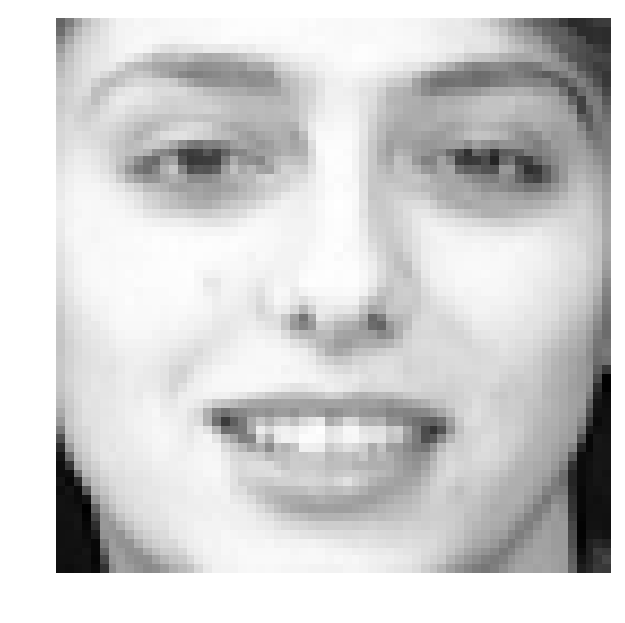
\includegraphics[width=60mm]{code/wienerimages/DeBlurImage.pdf}
	\caption{Deblurred image - image domain}
    \end{subfigure}%
   \begin{subfigure}[]{.5\textwidth}
   \centering   
        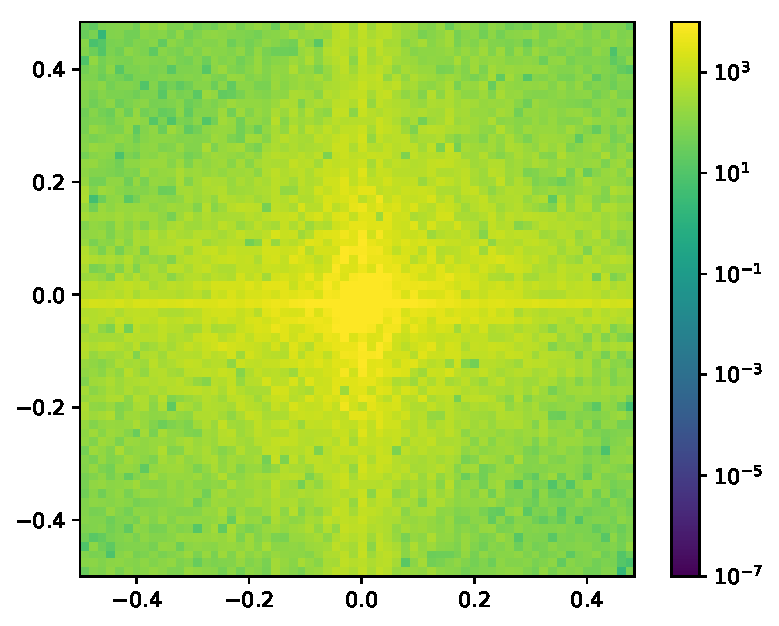
\includegraphics[width=60mm]{code/wienerimages/DeBlurImageFFT.pdf}
        \caption{Deblurred image - Fourier domain}
    \end{subfigure}% 
\end{figure}

	
 \item Apply your method to the image in the variable \texttt{noisy\_blur}, which contains a blurred image corrupted by some noise.  Report the result in the image and the Fourier domains (plot the magnitude of the Fourier coefficients). Explain what is happening.\\
 Using the same method as in part (a) we just spread the noise everywhere in time and frequency by multiplying to the inverse of the Gaussian noise (smoothing of noise).
 
  \begin{figure}[H] 
\captionsetup[subfigure]{labelformat=empty}
\centering
   \begin{subfigure}[]{.5\textwidth}
   \centering
        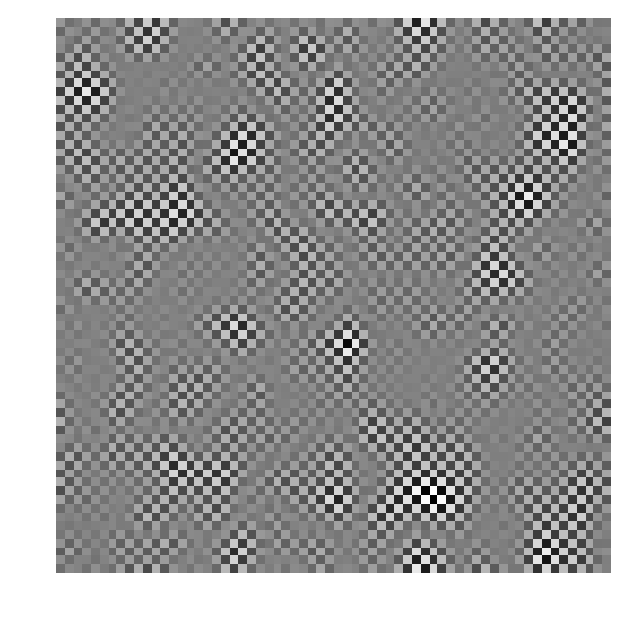
\includegraphics[width=60mm]{code/wienerimages/DeNoisyBlurImage.pdf}
	\caption{Deblurred noisy image - image domain}
    \end{subfigure}%
   \begin{subfigure}[]{.5\textwidth}
   \centering   
        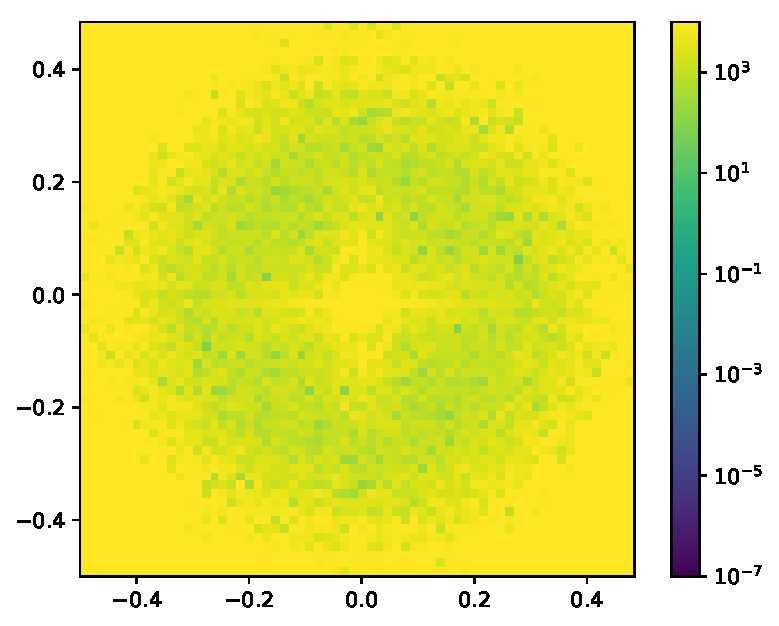
\includegraphics[width=60mm]{code/wienerimages/DeNoisyBlurImageFFT.pdf}
        \caption{Deblurred noisy image - Fourier domain}
    \end{subfigure}% 
\end{figure}


  \item Derive the Wiener filter for estimating a zero-mean vector $\ry$ from noisy blurred measurements $\rx = b \ast \ry + \rnd{z}$, where $b$ is a known blur kernel and $\rnd{z}$ is iid Gaussian noise with zero mean and variance $\sigma^2$. \\
  Using Theorem 5.3 from the stationarity notes, we have:
  \begin{align*}
  	\hat{w}[k]					&= 	\frac{\Cov(\rx_F[k], \ry_F[k])} {\Var(\rx_F[k])} \\
	\Cov(\rx_F[k], \ry_F[k])		&=	\E[\rx_F[k] \overline{\ry_F[k]}] \\
							&=	\E[(\rb_F[k] \ry_F[k] + \rnd{z}_F[k]) \; \overline{\ry_F[k]}] \\
							&=	\E[(\rb_F[k] \; \ry_F[k]  \overline{\ry_F[k]} ] + \E[ \rnd{z}_F[k]  \overline{\ry_F[k]}] \\
							&=	\rb_F[k]  \Var(\ry_F[k]) \\
	\Var(\rx_F[k]])				&=	\Var(\rb_F[k] \ry_F[k] + \rnd{z}_F[k])	\\
							&= 	\Var(\rb_F[k] \ry_F[k]) + \Var(\rnd{z}_F[k]) \text{ the cross-terms canceling out}\\
							&=	|\rb_F[k]|^2 \Var(\ry_F[k]) + N \sigma^2	\\	
	\hat{w}[k]					&= 	\frac{\rb_F[k]  \Var(\ry_F[k])} {|\rb_F[k]|^2 \Var(\ry_F[k]) + N \sigma^2}		
  \end{align*}
  
  
  \item Write a function \texttt{wiener\_deconvolution()} to recover the image from the noisy data (\texttt{noisy\_blur}). Report the result in the image and the Fourier domains (plot the magnitude of the Fourier coefficients). Compare this method to the result in (b) and explain why it works better. [Hint: you may have to use the variable \texttt{all\_images} and \texttt{s} here]\\
  Using the expression of the Wiener filter above and the statistics of all the images, we obtain a better result of deblurring the noisy image than the method described in part (a).
  We saw that in the above plots that most of the frequencies in the Fourier domain of  the true image are low frequencies, whereas deblurring the noisy image add high frequencies noise everywhere.
  Now if we look at the expression of the Fourier coefficients of the Wiener filter when multiplied with the DFT coefficients of the image, we observe that the Wiener coefficients go to $0$ for high-frequencies of the image which are quite small, leave unchanged frequencies of the signal not close to $0$ and in between multiply the Fourier coefficients of the image with a ratio smoothing the overall transition between these two sets of frequencies. One thing to note is our above calculations were assuming  a zero-mean vector for the measurements $\ry$ so before applying the Wiener filter in the Fourier domain we need to subtract the statistical mean from the noisy image, multiply by the Wiener coefficients, add the mean back before inverse transform the result in the image domain.
  
    \begin{figure}[H] 
\captionsetup[subfigure]{labelformat=empty}
\centering
   \begin{subfigure}[]{.5\textwidth}
   \centering
        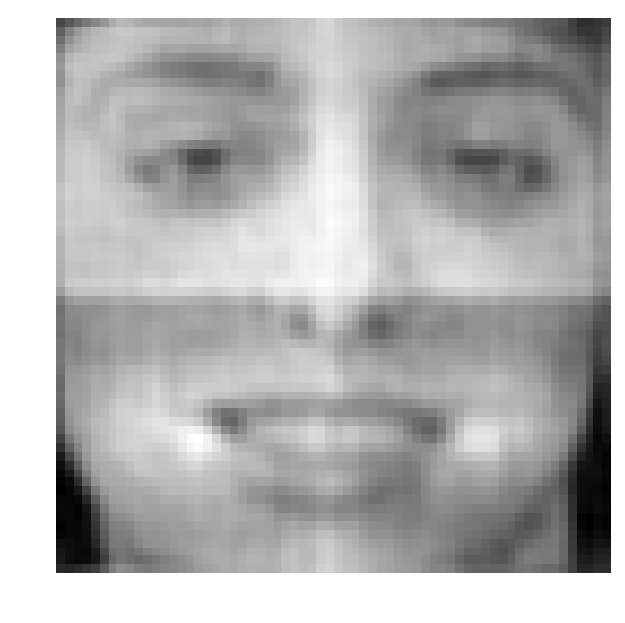
\includegraphics[width=60mm]{code/wienerimages/DeBlurNoisyImage.pdf}
	\caption{Deblurring with Wiener filter  - image domain}
    \end{subfigure}%
   \begin{subfigure}[]{.5\textwidth}
   \centering   
        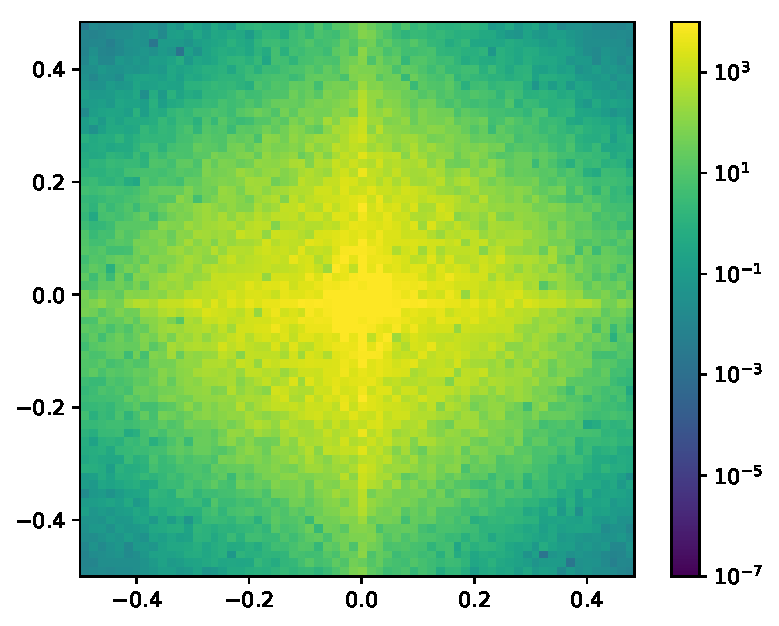
\includegraphics[width=60mm]{code/wienerimages/DeBlurNoisyImageFFT.pdf}
        \caption{Deblurring with Wiener filter - Fourier domain}
    \end{subfigure}% 
\end{figure}



  \end{enumerate}

 \end{enumerate}
\end{document}
